\documentclass[aspectratio=169, 10pt]{beamer}

\usetheme{Madrid}
\usecolortheme{whale}
\setbeamertemplate{navigation symbols}{}
\setbeamertemplate{footline}[frame number]

\usepackage[utf8]{inputenc}
\usepackage[T1]{fontenc}
\usepackage{graphicx}
\usepackage{booktabs}
\usepackage{amsmath}

\graphicspath{{figures/}{reports/figures/}}

\title[PAN 2025 GenAI Detection \& Attribution]{Multi-Level Stylometry \& N-Gram Baselines\\for Generative AI Detection and LLM Attribution}
\subtitle{Feature Extraction, Statistical Influence, and Dual-Task Baselines}
\author{Elia Gismondi}
\institute{Politecnico di Lodz --- PAN 2025 Shared Task 1}
\date{\today}

\begin{document}

% -------------------------------------------------------------------------
% SLIDE 1: TITLE
% -------------------------------------------------------------------------
\begin{frame}
    \titlepage
\end{frame}

% -------------------------------------------------------------------------
% SLIDE 2: STEPS 1 & 2 - FEATURE EXTRACTION & EXECUTION
% -------------------------------------------------------------------------
\begin{frame}{Steps 1 \& 2: Multi-Level Feature Space ($D = 4,600$)}
    \begin{columns}[c, onlytextwidth]
        \begin{column}{0.43\textwidth}
            \small
            \textbf{4 Feature Families} (Fit on Train only):
            \begin{itemize}\setlength\itemsep{2pt}
                \item \textbf{Stylometry (30):} TTR, Yule's $K$, Brunet's $W$, Honor\'e's $R$, lengths, 9 punct.\ ratios.
                \item \textbf{Function Words (70):} Closed-class relative frequencies (topic-invariant).
                \item \textbf{Char N-Grams (3,000):} \texttt{char\_wb} ($n=3..4$) sublinear TF-IDF.
                \item \textbf{Word N-Grams (1,500):} Lexical ($n=1..2$) TF-IDF with stop-words.
            \end{itemize}
            \vspace{0.15cm}
            \textbf{Corpus Execution \& Audit:}
            \begin{itemize}\setlength\itemsep{2pt}
                \item \textbf{Train:} $23,707 \times 4,600$ ($417\text{ docs/s}$)
                \item \textbf{Val:} $3,589 \times 4,600$ ($514\text{ docs/s}$)
                \item \textbf{Audit:} 63.2\% sparsity, \textbf{0 NaN / 0 Inf}
            \end{itemize}
        \end{column}
        \begin{column}{0.55\textwidth}
            \centering
            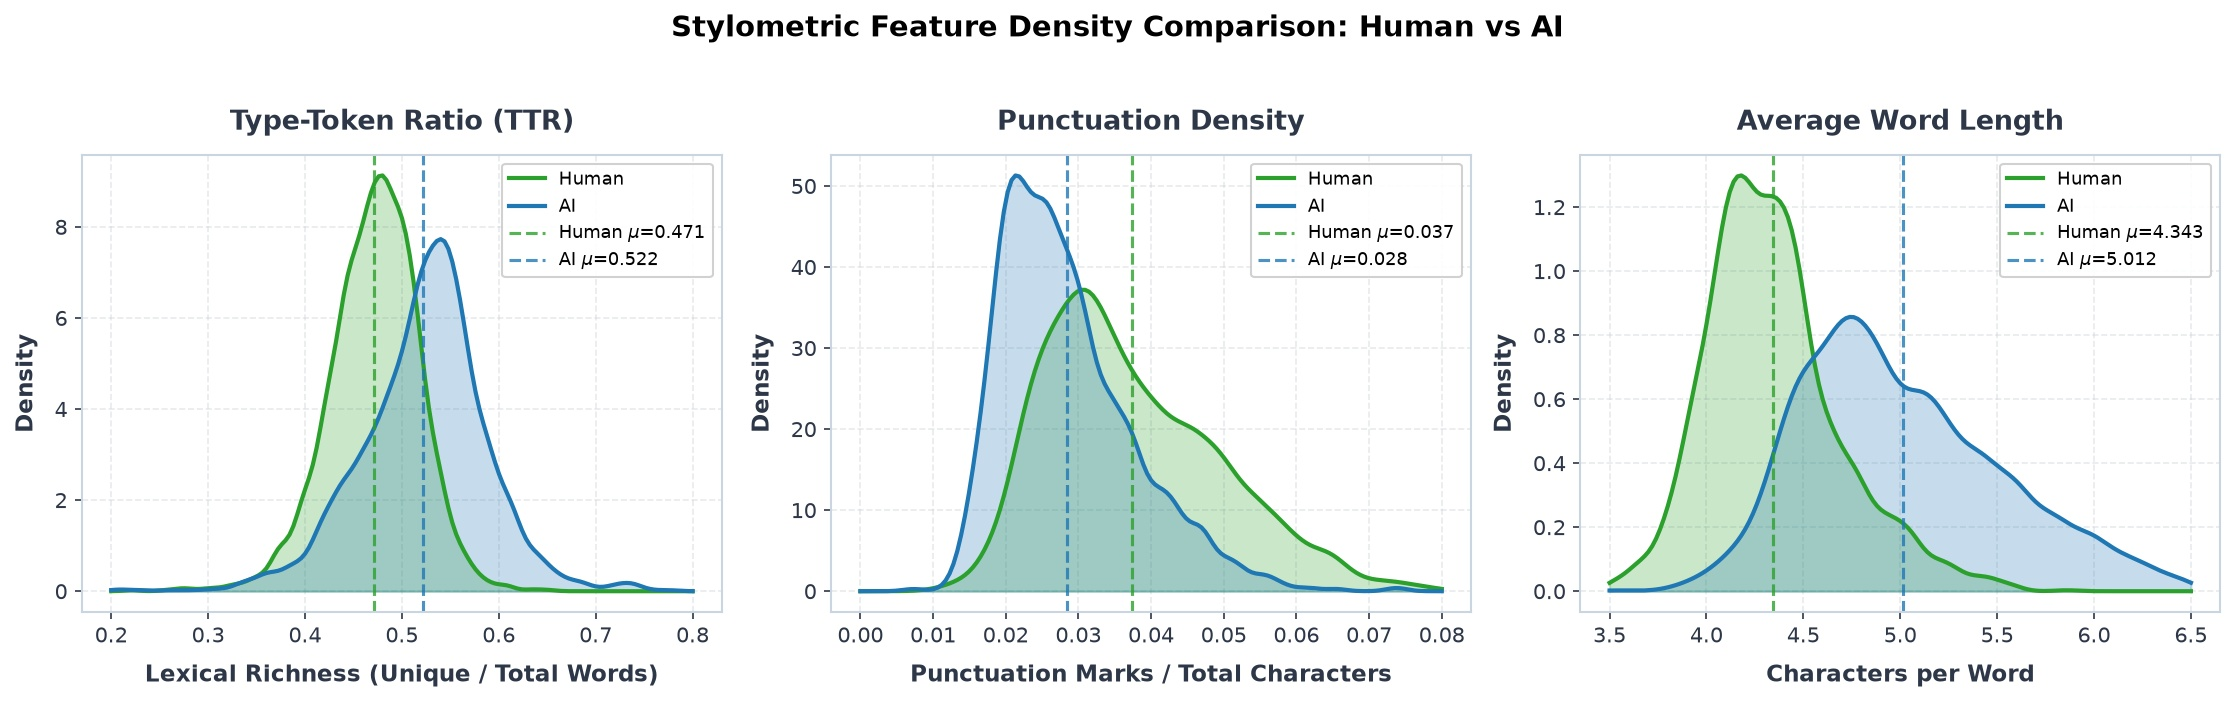
\includegraphics[width=\linewidth, height=0.72\textheight, keepaspectratio]{stylometric_distributions}
        \end{column}
    \end{columns}
\end{frame}

% -------------------------------------------------------------------------
% SLIDE 3: STEP 3A - FEATURE INFLUENCE ON BINARY OUTPUT
% -------------------------------------------------------------------------
\begin{frame}{Step 3A: Feature Influence on Binary Output ($y \in \{0, 1\}$)}
    \centering
    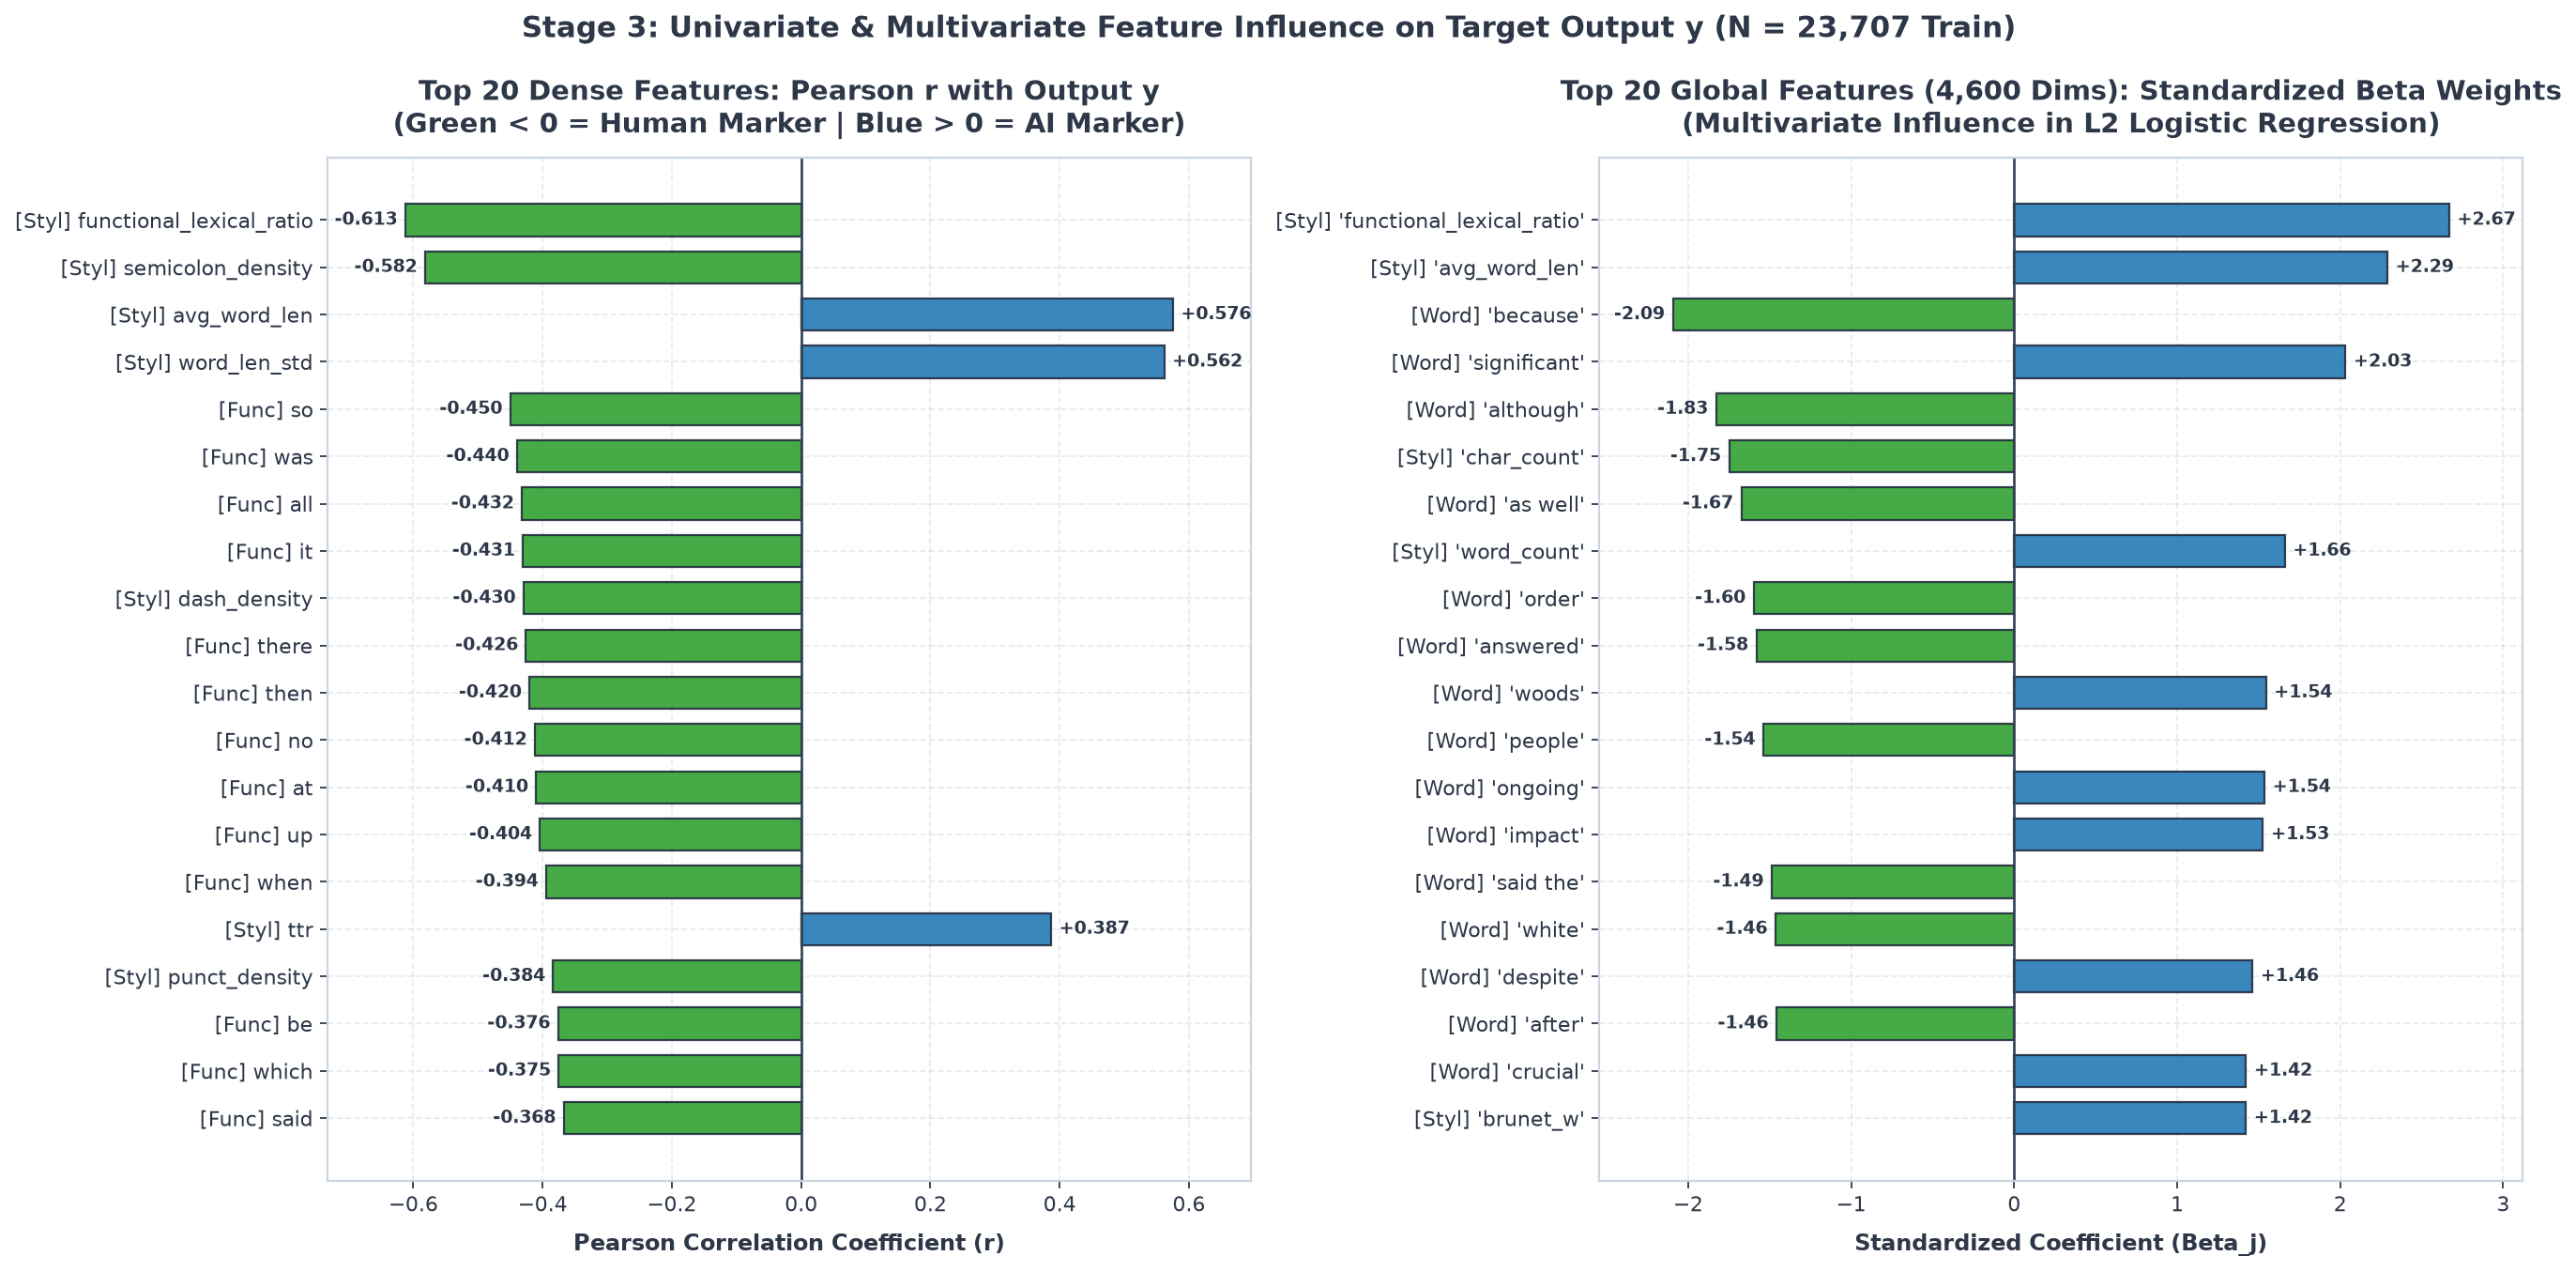
\includegraphics[width=0.92\textwidth, height=0.62\textheight, keepaspectratio]{feature_influence_comprehensive.png}
    \vspace{0.1cm}
    \small
    \begin{itemize}\setlength\itemsep{1pt}
        \item \textbf{Top Human Markers ($r < 0, \beta < 0$):} \texttt{functional\_lexical\_ratio} ($r=-0.613$), \texttt{semicolon\_density} ($r=-0.582$), \texttt{dash\_density} ($r=-0.430$), \textit{``because''} ($\beta=-2.09$).
        \item \textbf{Top AI Markers ($r > 0, \beta > 0$):} \texttt{avg\_word\_len} ($r=+0.576$, \textbf{$-14.1\%$ Permutation F1 drop}), \texttt{ttr} ($r=+0.387$), RLHF terms (\textit{``significant''}, \textit{``ongoing''}, \textit{``impact''}, \textit{``crucial''}).
    \end{itemize}
\end{frame}

% -------------------------------------------------------------------------
% SLIDE 4: STEP 3B - FEATURE INFLUENCE FOR LLM ATTRIBUTION
% -------------------------------------------------------------------------
\begin{frame}{Step 3B: Discriminating Across 22 AI Models (Multiclass ANOVA)}
    \begin{columns}[c, onlytextwidth]
        \begin{column}{0.38\textwidth}
            \small
            \textbf{Top Discriminators ($F$-stat):}
            \begin{itemize}\setlength\itemsep{1.5pt}
                \item \texttt{uppercase\_ratio} ($F=700$)
                \item \texttt{root\_ttr} ($F=530$) \& \texttt{ttr} ($F=379$)
                \item \texttt{hapax\_ratio} ($F=462$)
                \item \texttt{brunet\_w} ($F=401$)
                \item \texttt{char\_count} ($F=340$)
                \item \texttt{comma\_density} ($F=337$)
            \end{itemize}
            \vspace{0.15cm}
            \textbf{Vendor Signatures:}
            \begin{itemize}\setlength\itemsep{1.5pt}
                \item \textbf{OpenAI:} High TTR ($+0.65z$), low comma density ($-0.50z$).
                \item \textbf{DeepSeek:} Longest outputs ($+0.80z$).
                \item \textbf{Falcon:} Highest hapax ($+0.73z$).
            \end{itemize}
        \end{column}
        \begin{column}{0.60\textwidth}
            \centering
            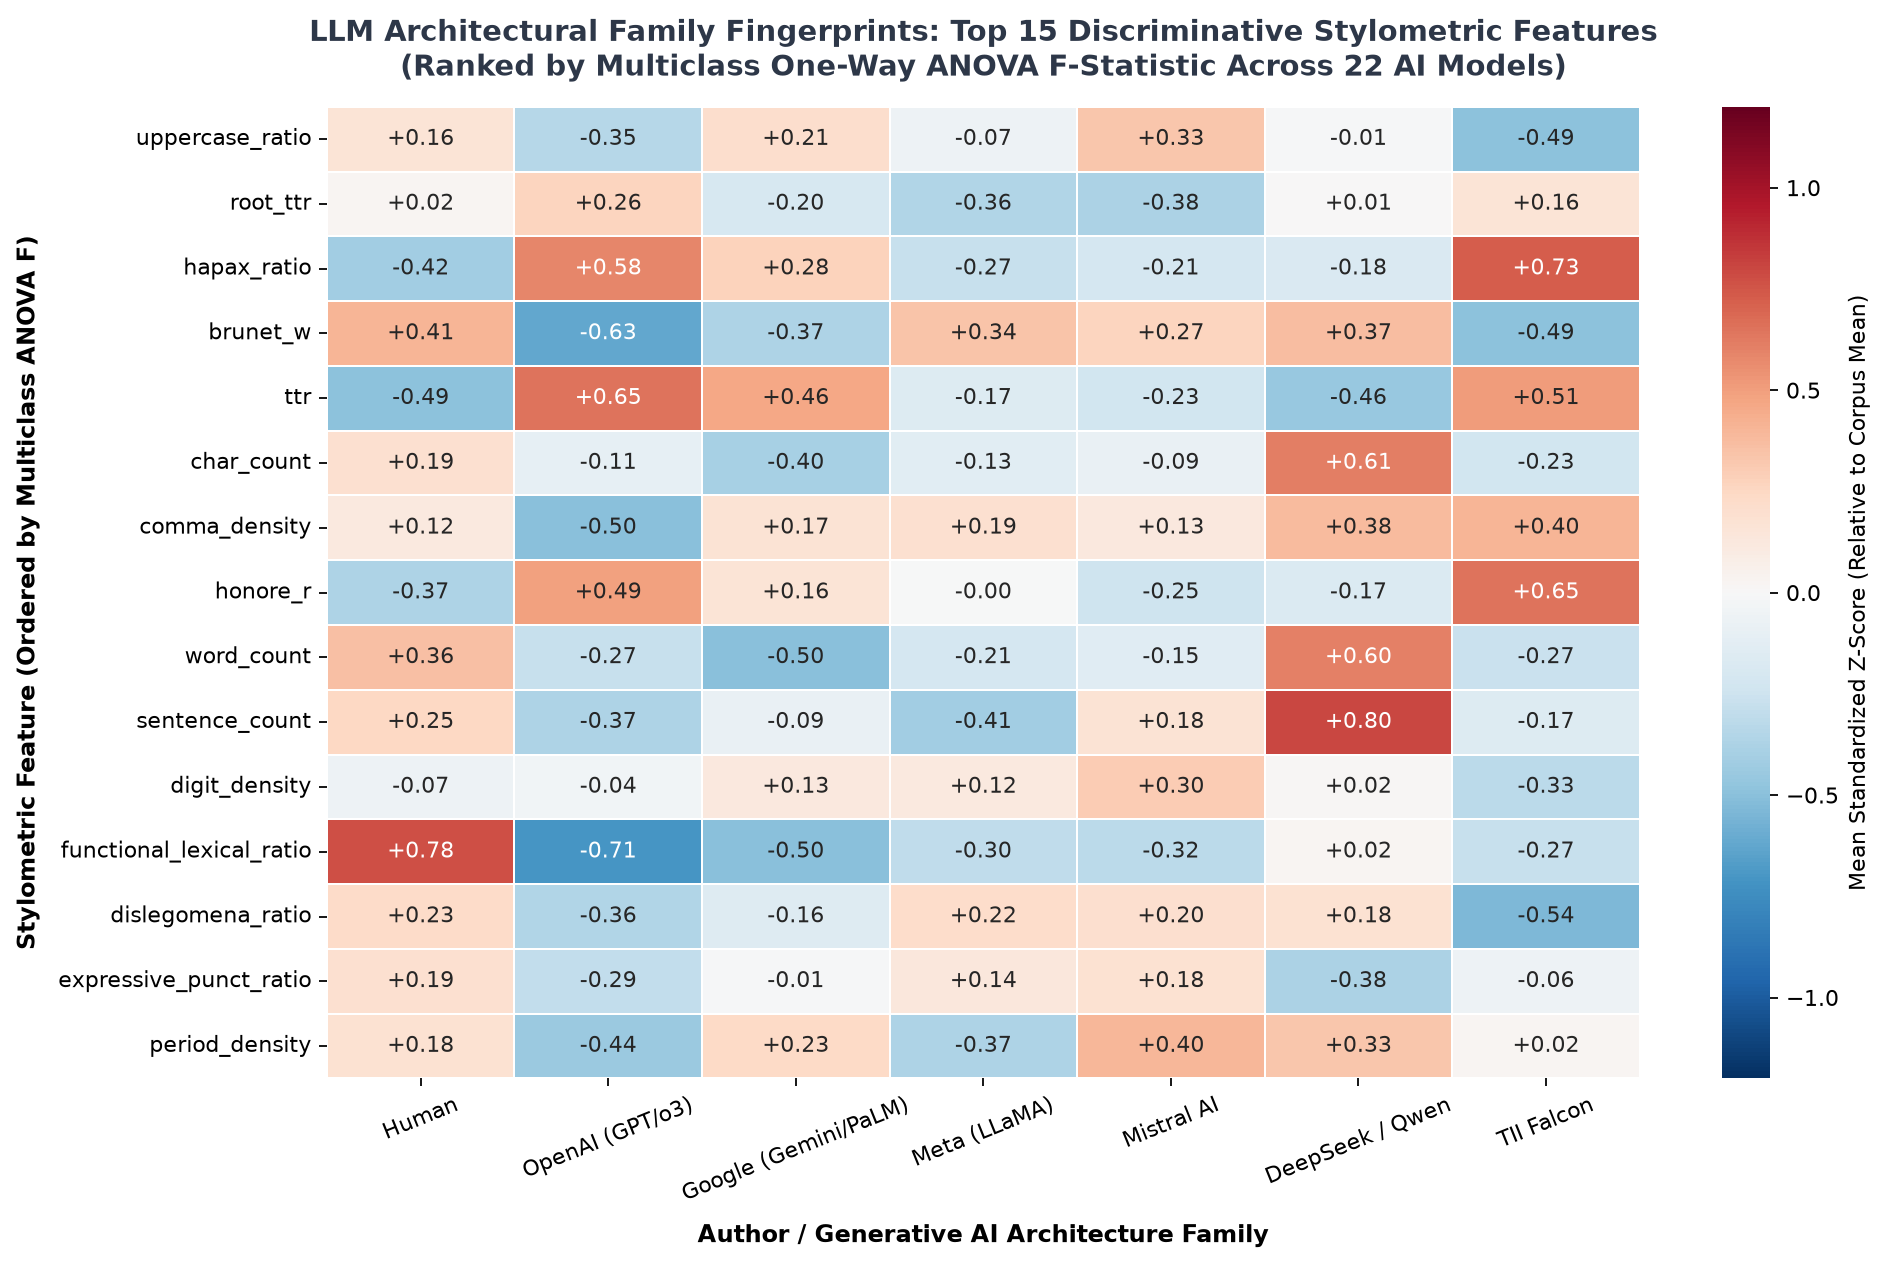
\includegraphics[width=\linewidth, height=0.75\textheight, keepaspectratio]{llm_family_stylometric_fingerprints.png}
        \end{column}
    \end{columns}
\end{frame}

% -------------------------------------------------------------------------
% SLIDE 5: STEP 3C - FEATURE FAMILY ABLATION STUDY
% -------------------------------------------------------------------------
\begin{frame}{Step 3C: Feature Family Ablation \& Leave-One-Out Impact}
    \centering
    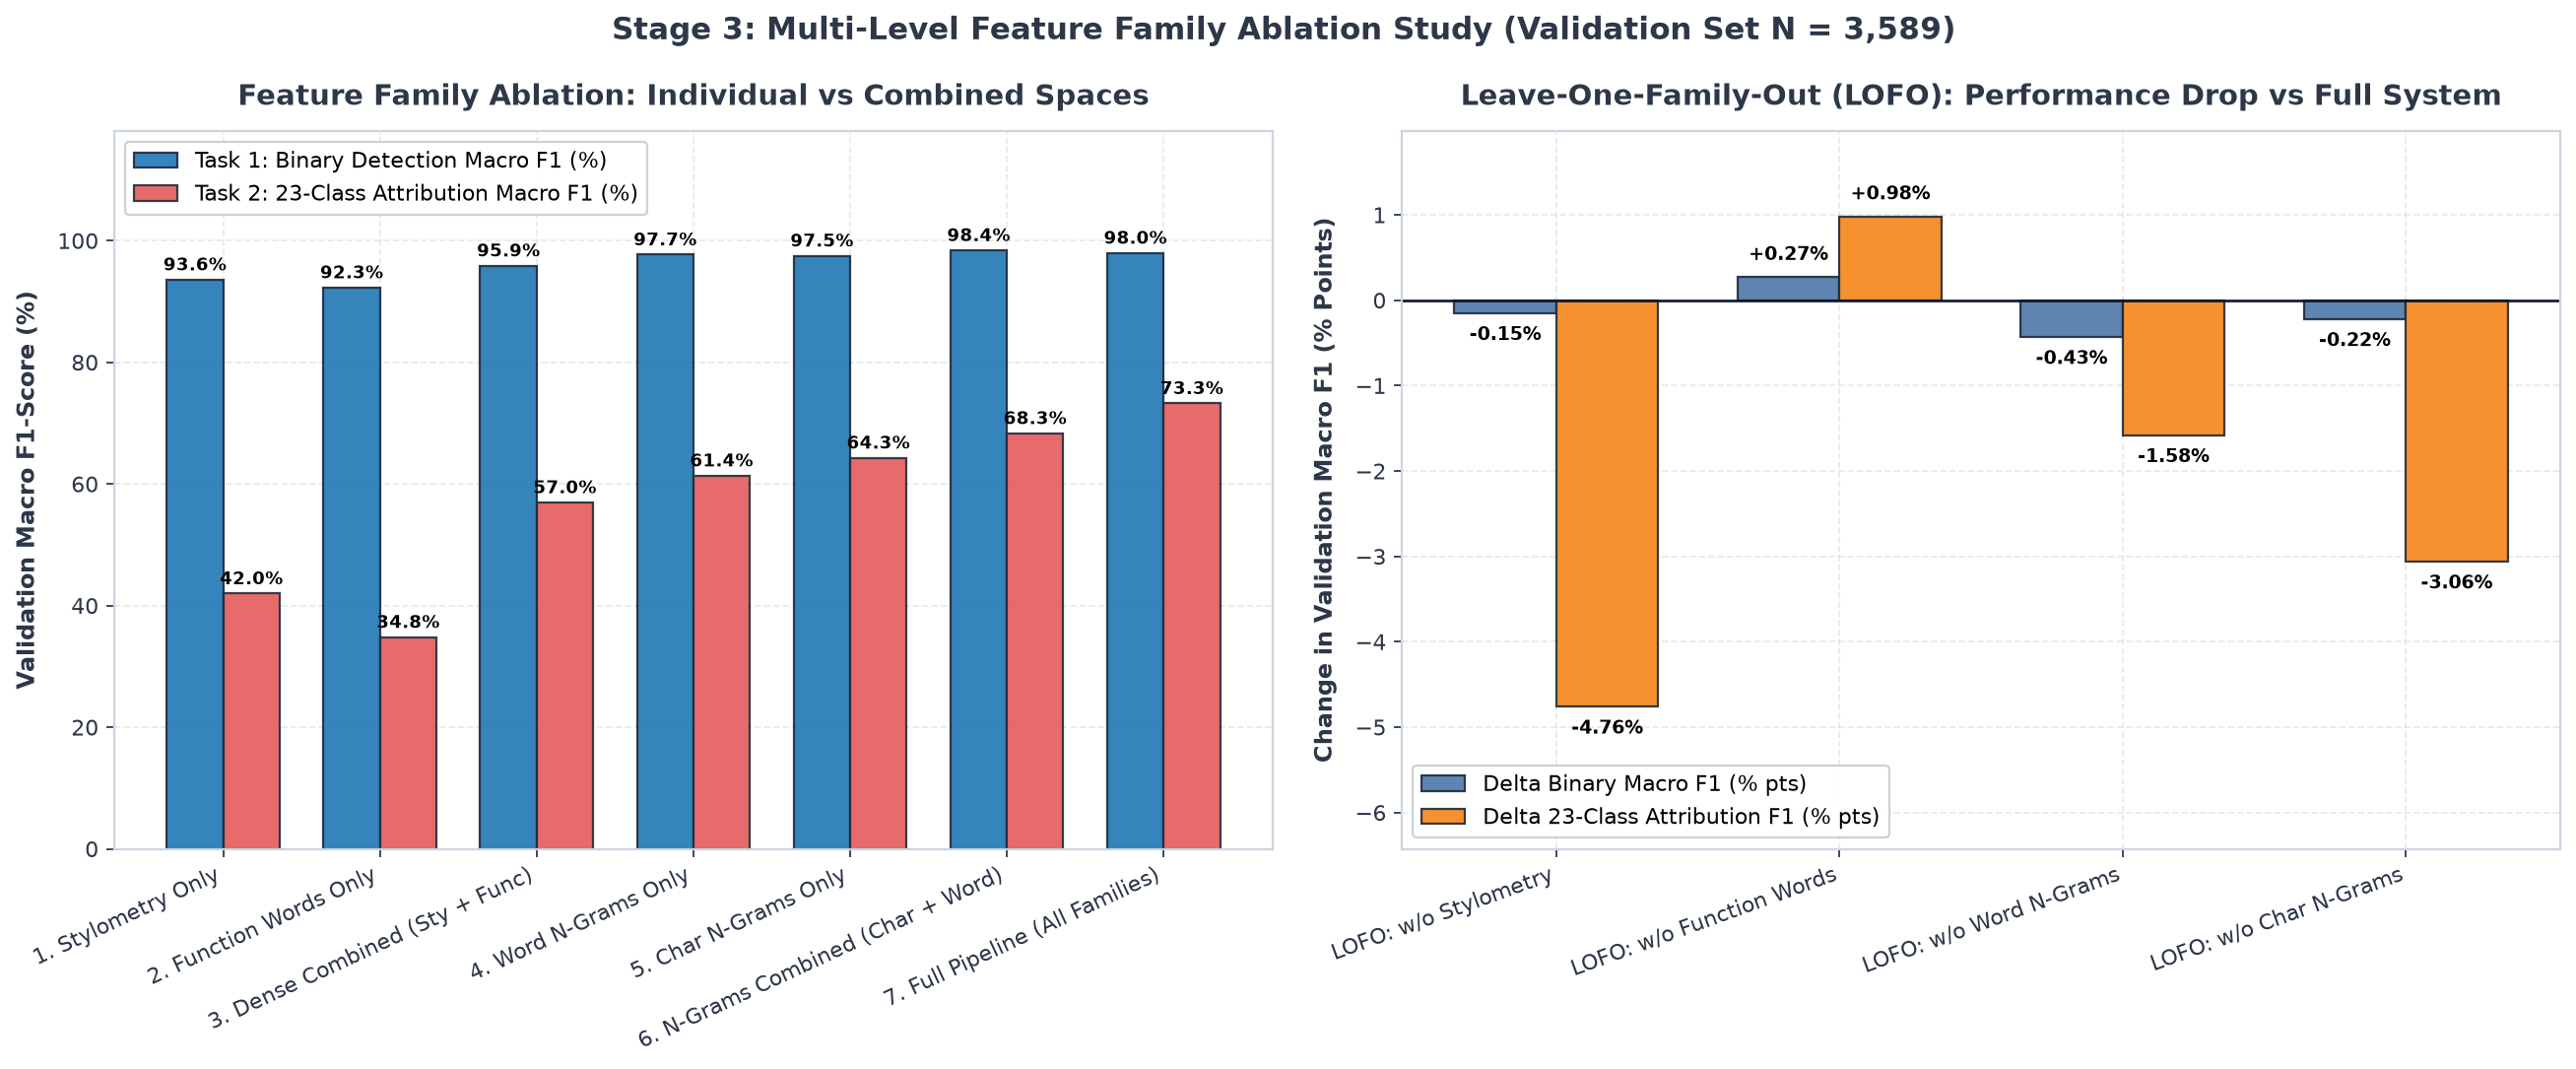
\includegraphics[width=0.94\textwidth, height=0.64\textheight, keepaspectratio]{feature_family_ablation.png}
    \vspace{0.1cm}
    \small
    \begin{itemize}\setlength\itemsep{1pt}
        \item \textbf{Stylometry Alone (30 dims):} Achieves \textbf{93.61\% Binary Macro F1} (97.91\% ROC-AUC).
        \item \textbf{Synergy on 23-Class Attribution:} Removing Stylometry causes the largest drop (\textbf{$-4.76\%$ Macro F1}), followed by Char N-Grams (\textbf{$-3.06\%$}). Full pipeline reaches \textbf{73.27\% Macro F1}.
    \end{itemize}
\end{frame}

% -------------------------------------------------------------------------
% SLIDE 6: STEP 4A - DUAL-TASK BASELINE BENCHMARK
% -------------------------------------------------------------------------
\begin{frame}{Step 4A: Dual-Task Baseline Models Benchmark ($N_{\text{val}} = 3,589$)}
    \centering
    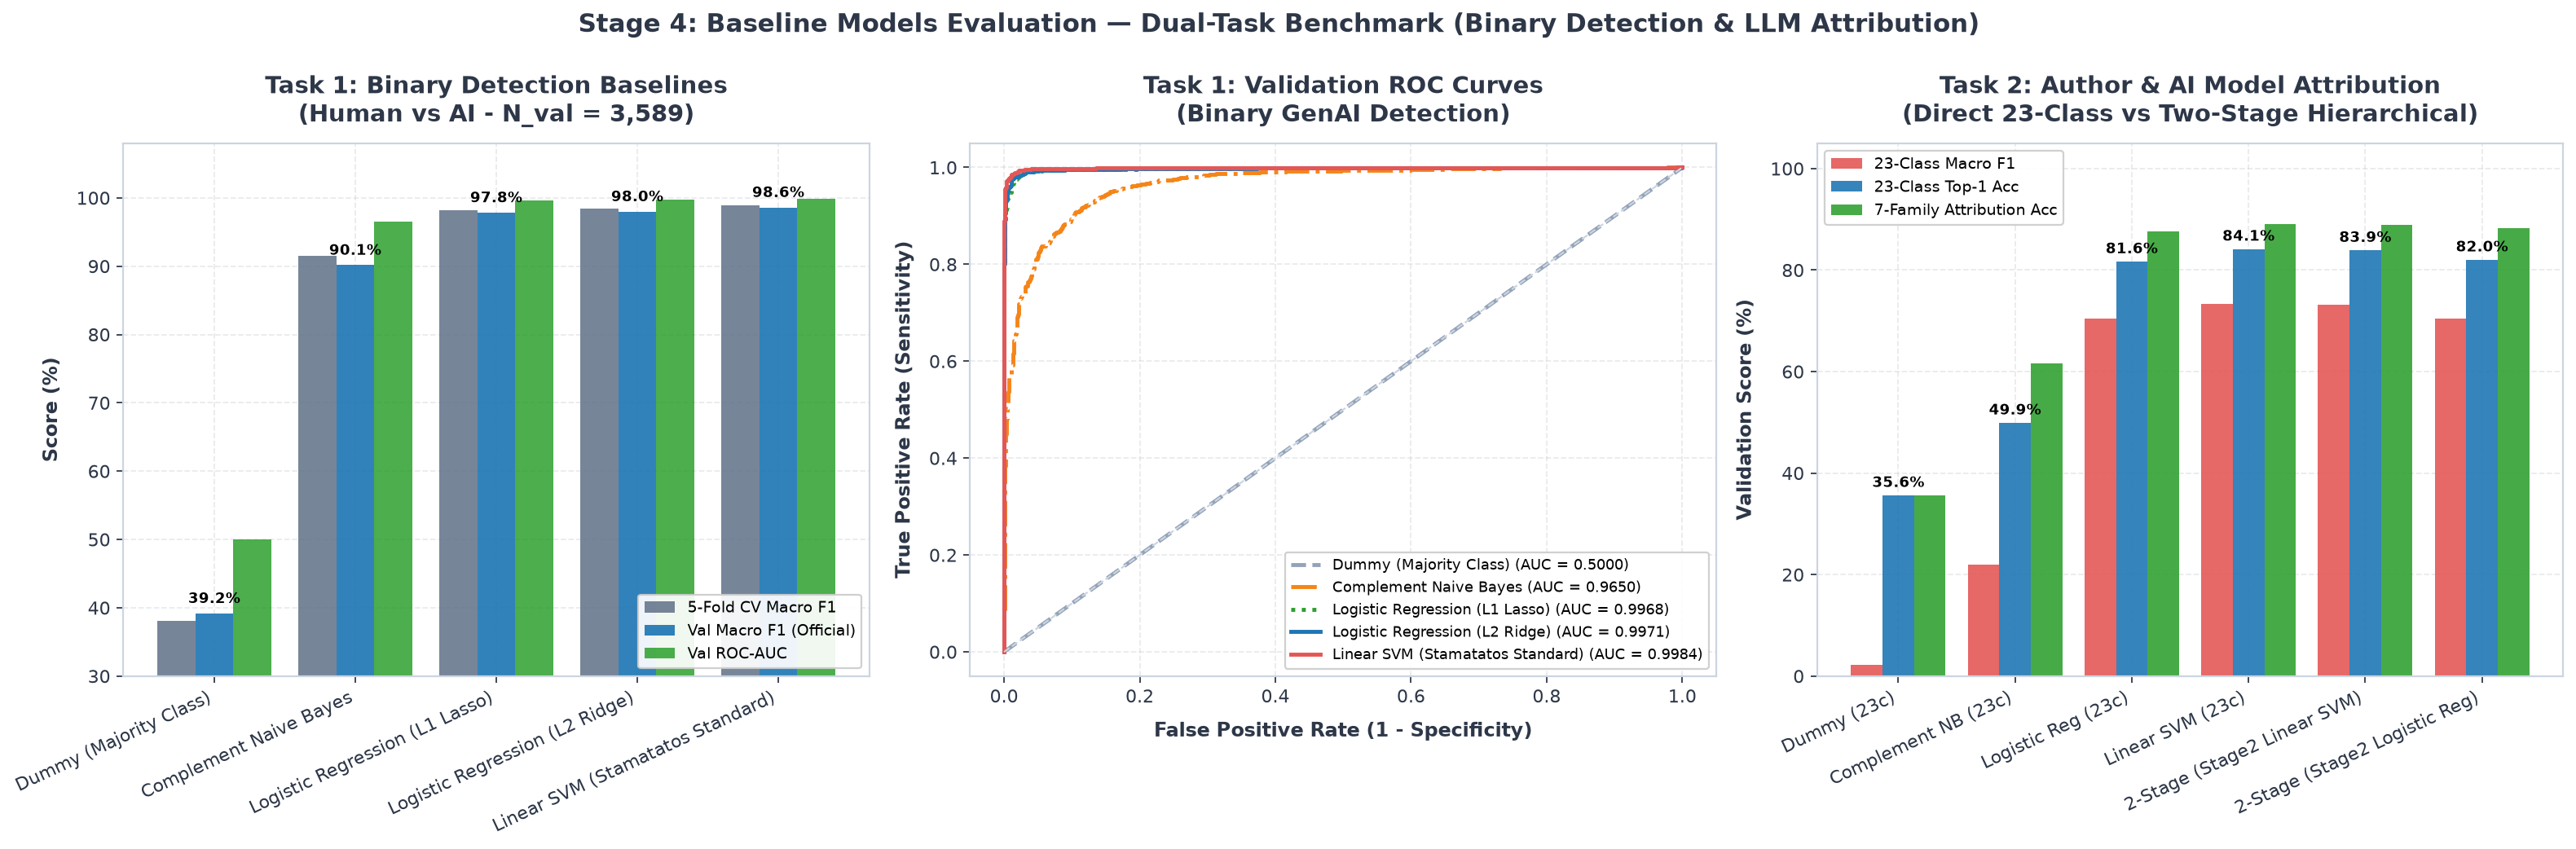
\includegraphics[width=0.96\textwidth, height=0.48\textheight, keepaspectratio]{baseline_models_benchmark.png}
    \vspace{0.08cm}
    \scriptsize
    \begin{tabular}{lcccc|ccc}
        \toprule
        \textbf{Baseline Model} & \textbf{CV5 F1} & \textbf{Val Bin F1} & \textbf{ROC-AUC} & \textbf{FP / FN} & \textbf{23c Top-1} & \textbf{23c Top-3} & \textbf{7-Fam Acc} \\
        \midrule
        Dummy (Majority) & 38.1\% & 39.2\% & 50.0\% & 1277 / 0 & 35.6\% & 39.3\% & 35.6\% \\
        Complement NB & 91.6\% & 90.2\% & 96.5\% & 178 / 144 & 49.9\% & 69.5\% & 61.6\% \\
        Logistic Reg (L2) & 98.5\% & 98.0\% & 99.7\% & 40 / 26 & 81.6\% & 94.6\% & 87.7\% \\
        \textbf{Linear SVM} & \textbf{98.9\%} & \textbf{98.6\%} & \textbf{99.8\%} & \textbf{26 / 20} & \textbf{84.1\%} & \textbf{94.9\%} & \textbf{89.1\%} \\
        \textbf{Two-Stage SVM} & --- & \textbf{98.6\%} & \textbf{99.8\%} & \textbf{26 / 20} & 83.9\% & 94.0\% & \textbf{88.9\% (83.1\% F1)} \\
        \bottomrule
    \end{tabular}
\end{frame}

% -------------------------------------------------------------------------
% SLIDE 7: STEP 4B - CONFUSION MATRICES & CROSS-GENRE DIAGNOSTICS
% -------------------------------------------------------------------------
\begin{frame}{Step 4B: Confusion Matrices \& Cross-Domain Generalization}
    \centering
    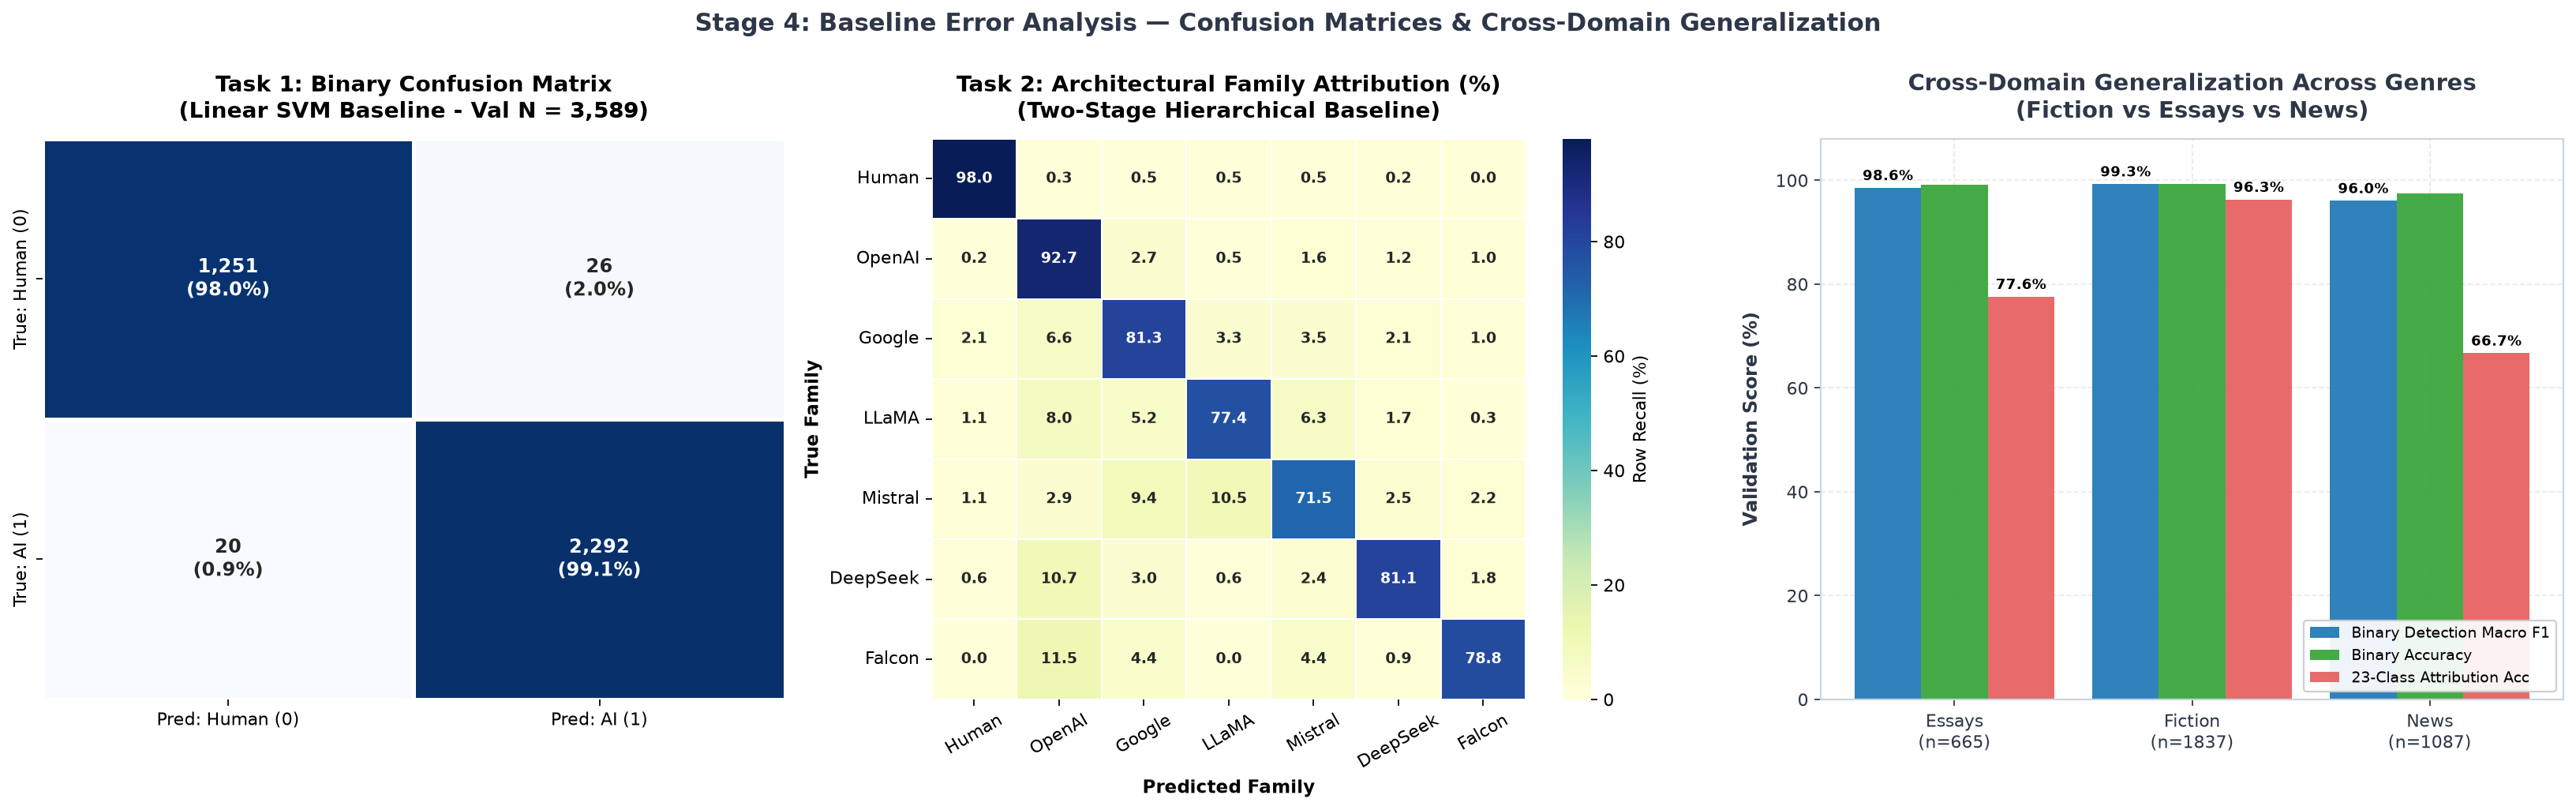
\includegraphics[width=0.96\textwidth, height=0.62\textheight, keepaspectratio]{baseline_diagnostics_and_confusion.png}
    \vspace{0.1cm}
    \small
    \begin{itemize}\setlength\itemsep{1pt}
        \item \textbf{Binary Recall:} \textbf{98.0\%} on Human ($1,251/1,277$) and \textbf{99.1\%} on AI ($2,292/2,312$).
        \item \textbf{Cross-Genre Stability:} High binary F1 across \textbf{Fiction (99.3\%)}, \textbf{Essays (98.6\%)}, and \textbf{News (96.1\%)}; 23-class attribution peaks in Fiction (\textbf{96.3\%}).
    \end{itemize}
\end{frame}

% -------------------------------------------------------------------------
% SLIDE 8: STEP 4C - PER-LLM ATTRIBUTION & FINGERPRINTING
% -------------------------------------------------------------------------
\begin{frame}{Step 4C: Per-Author \& Per-LLM Detection and Attribution}
    \begin{columns}[c, onlytextwidth]
        \begin{column}{0.38\textwidth}
            \small
            \textbf{Key Takeaways:}
            \begin{itemize}\setlength\itemsep{4pt}
                \item \textbf{Zero Evasion:} \textbf{100\% Binary Recall} on 13 out of 22 AI models.
                \item \textbf{Top Exact Attribution (23c):}\\
                \texttt{human} (\textbf{98.0\%}), \texttt{o3-mini} (\textbf{97.7\%}), \texttt{gpt-4.5} (\textbf{95.6\%}), \texttt{gpt-4o-mini} (\textbf{90.7\%}), \texttt{llama-3.3-70b} (\textbf{88.9\%}), \texttt{gemini-2.0} (\textbf{88.5\%}).
                \item \textbf{Intra-Family Confusion:}\\
                Misclassifications occur almost exclusively between sibling models (\texttt{gpt-4-turbo} $\leftrightarrow$ \texttt{gpt-4o}, \texttt{llama-2-7b} $\leftrightarrow$ \texttt{70b}).
            \end{itemize}
        \end{column}
        \begin{column}{0.60\textwidth}
            \centering
            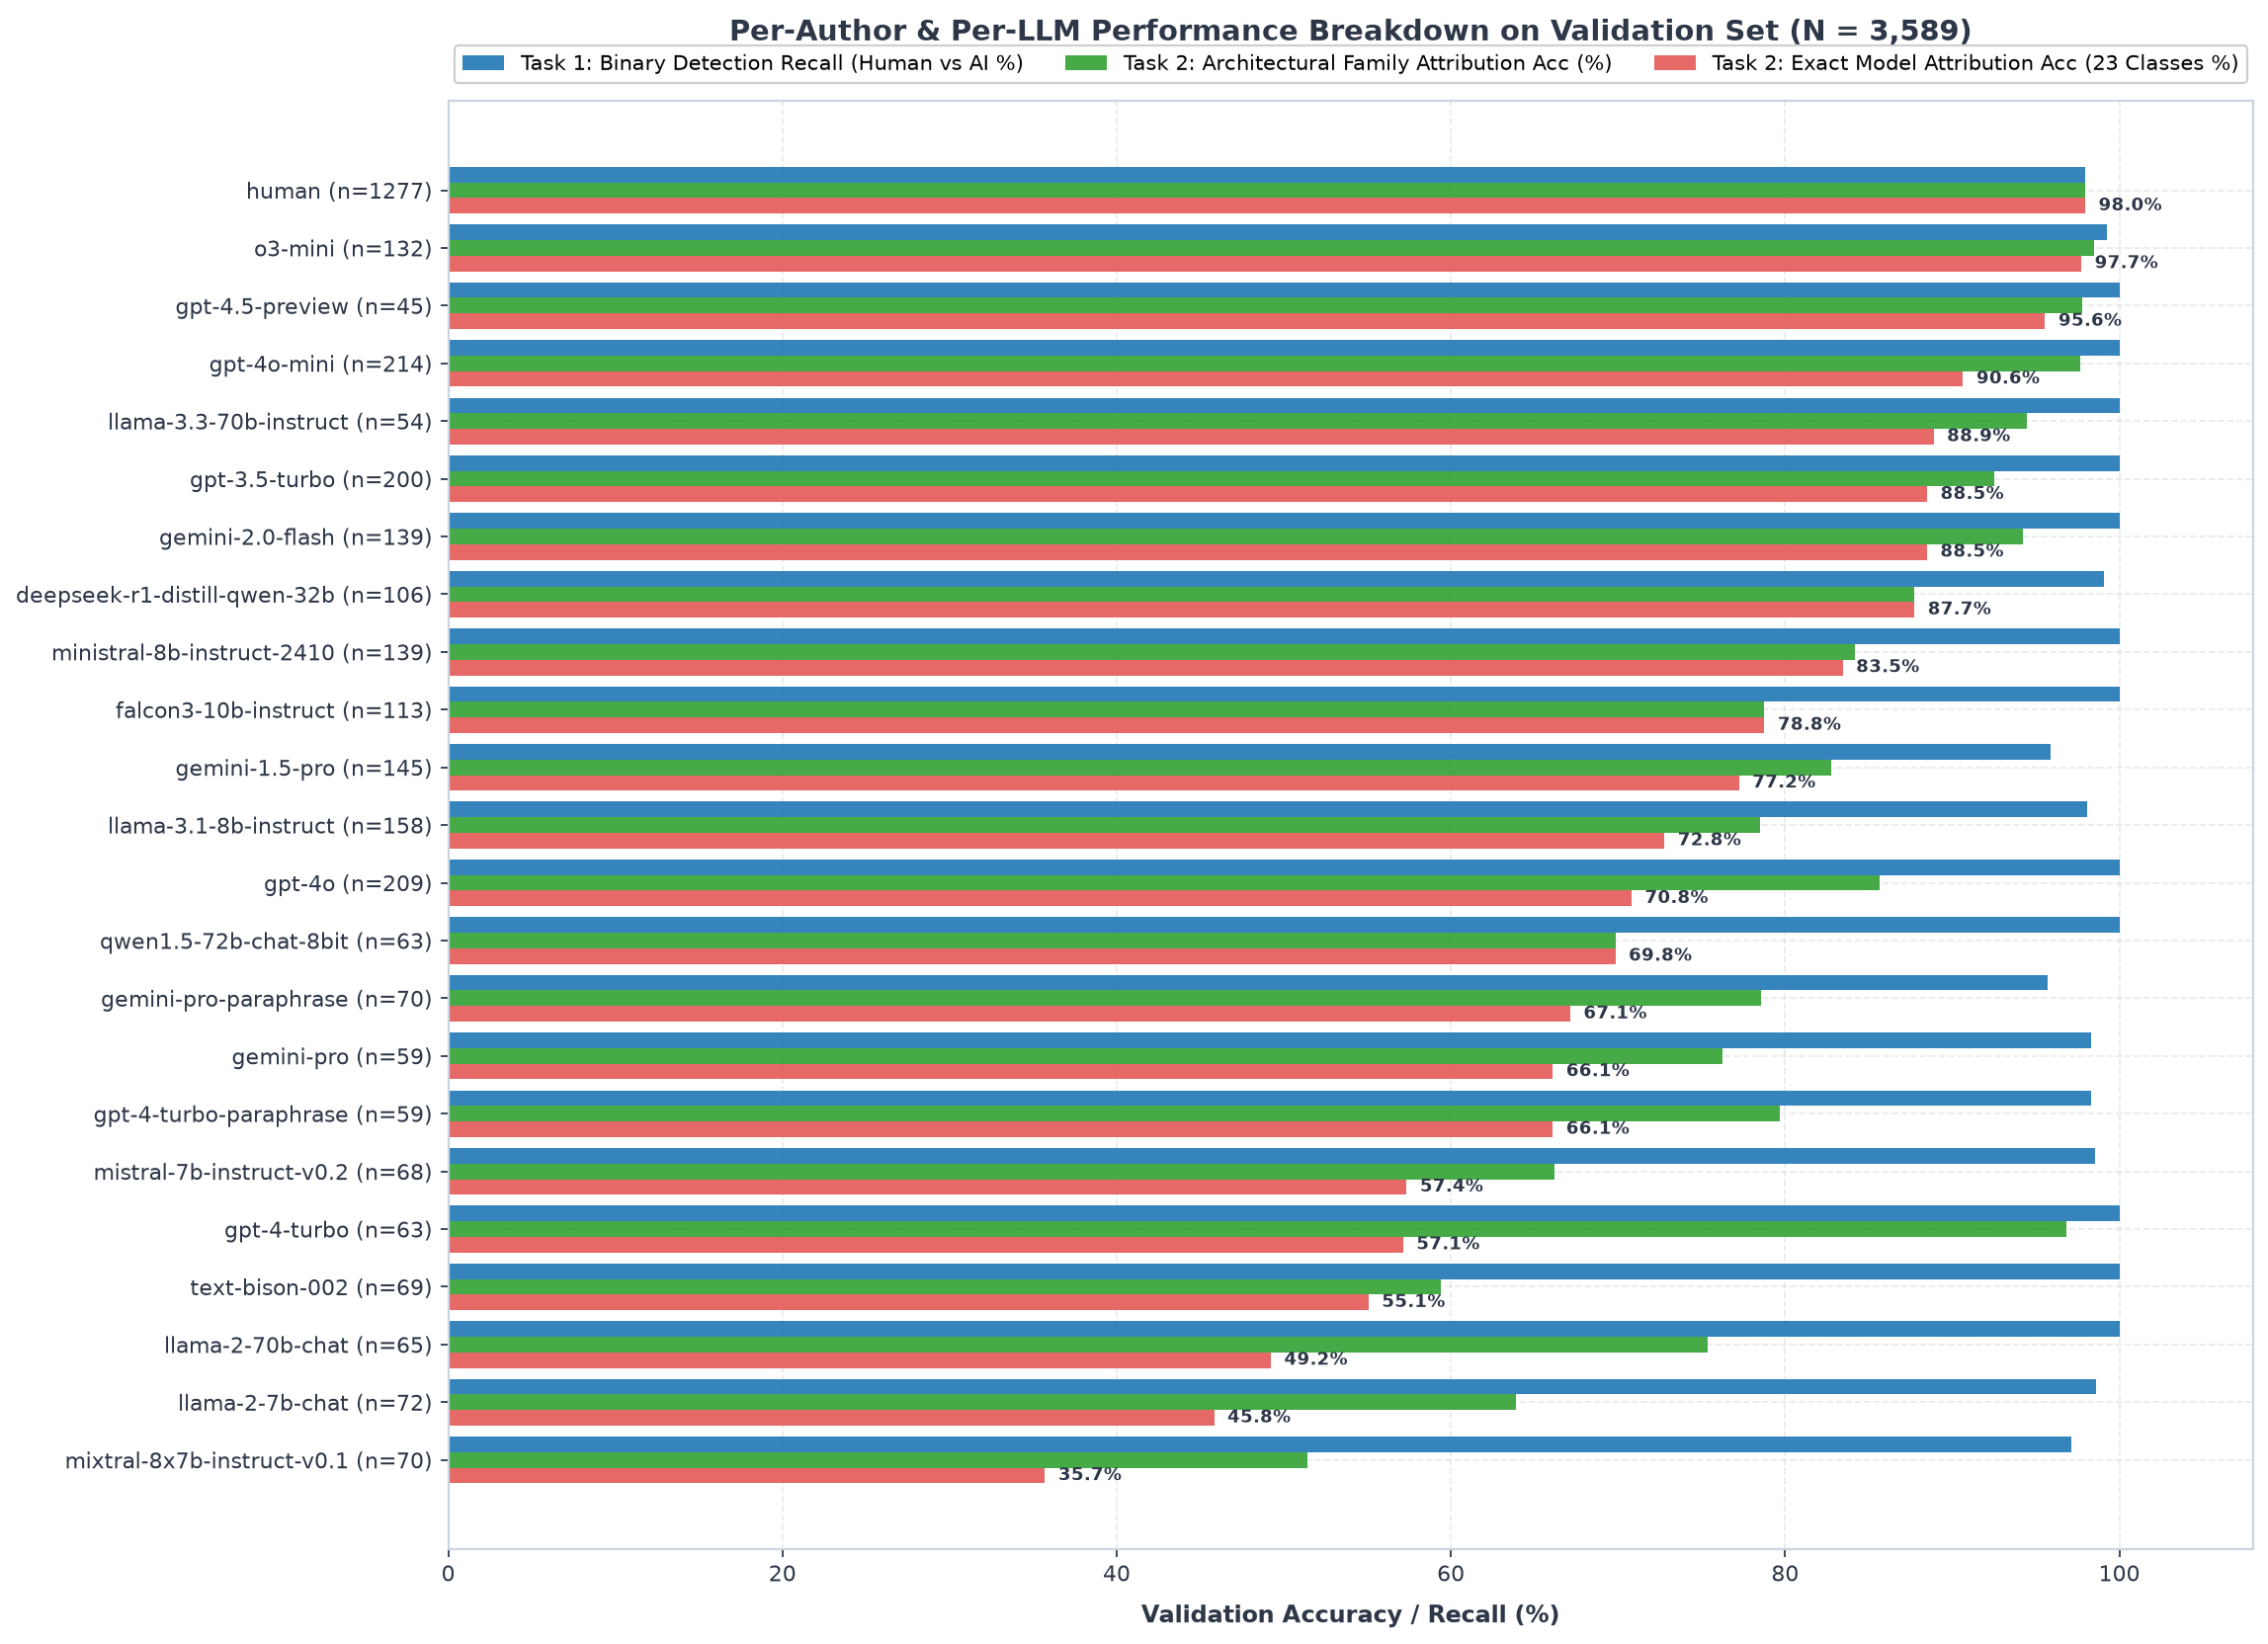
\includegraphics[width=\linewidth, height=0.75\textheight, keepaspectratio]{per_llm_detection_and_attribution.png}
        \end{column}
    \end{columns}
\end{frame}

\end{document}
